\documentclass[11pt]{article}
\usepackage{geometry,marginnote} % Pour passer au format A4
\geometry{hmargin=1cm, vmargin=1.5cm} % 

% Page et encodage
\usepackage[T1]{fontenc} % Use 8-bit encoding that has 256 glyphs
\usepackage[english,french]{babel} % Français et anglais
\usepackage[utf8]{inputenc} 

\usepackage{lmodern}
\usepackage[np]{numprint}
\setlength\parindent{0pt}

% Graphiques
\usepackage{graphicx,float,grffile}
\usepackage{tikz,pst-eucl,pst-plot,pstricks,pst-node,pstricks-add,pst-fun,pgfplots} 

% Maths et divers
\usepackage{amsmath,amsfonts,amssymb,amsthm,verbatim,scratch3}
\usepackage{multicol,enumitem,url,eurosym,gensymb,tabularx}

\DeclareUnicodeCharacter{20AC}{\euro}



% Sections
\usepackage{sectsty} % Allows customizing section commands
\allsectionsfont{\centering \normalfont\scshape}

% Tête et pied de page
\usepackage{fancyhdr} \pagestyle{fancy} \fancyhead{} \fancyfoot{}

%\fancyfoot[L]{Collège Faubert}
%\fancyfoot[C]{\thepage / 6}
%\fancyfoot[R]{Série Générale}

\renewcommand{\headrulewidth}{0pt} % Remove header underlines
%\renewcommand{\footrulewidth}{0pt} % Remove footer underlines

\newcommand{\horrule}[1]{\rule{\linewidth}{#1}} % Create horizontal rule command with 1 argument of height

\newcommand{\Pointilles}[1][3]{%
  \multido{}{#1}{\makebox[\linewidth]{\dotfill}\\[\parskip]
}}

\newtheorem{Definition}{Définition}

\usepackage{siunitx}
\sisetup{
    detect-all,
    output-decimal-marker={,},
    group-minimum-digits = 3,
    group-separator={~},
    number-unit-separator={~},
    inter-unit-product={~}
}

\setlength{\columnseprule}{1pt}

\setlength{\columnseprule}{0pt}

\begin{document}

\begin{center}
  \textit{Le plus grand ennemi de la connaissance n'est pas l'ignorance. C'est l'illusion de la connaissance.} 
  
  \textbf{Stephen Hawking}
\end{center}


\subsection*{Exercice 1 - Calculer}

\begin{itemize}[label={$\bullet$}]
  \item $ 100 - (-45) $
  \item $ 50 \times (-3) $
  \item $ -45 + (-45) $
  \item $ -2 \times (-13) $
  \item $ -111 + 111 $
  \item $ -64 - 38 $ 
\end{itemize}


\subsection*{Exercice 2 - Calculer}
\textit{faire des étapes}

\begin{itemize}[label={$\bullet$}]
  \item $ 120 + 5 \times -11$
  \item $(10 - 14) \times (14 - 6)$
  \item $-140 + 2 \times (12 - 22)$
  \item $24 - 11 \times (41 + (-22))$
\end{itemize}

\subsection*{Programme de calcul 1}

\fbox{%
\begin{minipage}{0.75\textwidth}
\begin{itemize}[label={$\bullet$}]
  \item Choisir un nombre.
  \item Ajouter 15 au nombre de départ. 
  \item Multiplier par 3 le résultat précédent.
  \item Soustraire 45 au résultat précédent.
\end{itemize} 
\end{minipage}
}

\begin{enumerate}
  \item[1.] On choisit $10$ comme nombre de départ. \newline Quel est le résultat à la fin du programme ?
  \item[2.] On choisit $-12$ comme nombre de départ. \newline Quel est le résultat à la fin du programme ?
\end{enumerate}

\subsection*{Programme de calcul 2}

\fbox{%
\begin{minipage}{0.75\textwidth}
\begin{itemize}[label={$\bullet$}]
  \item Choisir un nombre.
  \item Ajouter 6 au nombre de départ. 
  \item Soustraire 6 au nombre de départ.
  \item Multiplier les deux résultats précédents.
\end{itemize} 
\end{minipage}
}

\begin{enumerate}
  \item[1.] On choisit $10$ comme nombre de départ. \newline Quel est le résultat à la fin du programme ?
  \item[2.] On choisit $-12$ comme nombre de départ. \newline Quel est le résultat à la fin du programme ?
\end{enumerate}

\newpage

\begin{multicols}{4}
\begin{figure}[H]
  \centering
  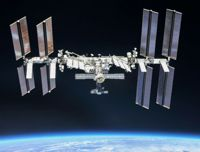
\includegraphics[width=100px]{4x2-nombres-relatifs/ex4.jpg}
\end{figure}

\begin{figure}[H]
  \centering
  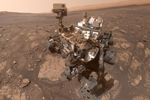
\includegraphics[width=100px]{4x2-nombres-relatifs/ex5.jpg}
\end{figure}

\begin{figure}[H]
  \centering
  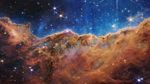
\includegraphics[width=100px]{4x2-nombres-relatifs/ex6.jpg}
\end{figure}

\begin{figure}[H]
  \centering
  
\includegraphics[width=100px]{4x2-nombres-relatifs/ex2.jpg}
\end{figure}
\end{multicols}

\vspace{1cm}

\subsection*{PB1 : Mars} 

Sur Mars, la température le jour est de $27\degree C$ et la nuit de $-84\degree C$.\\

Quelle est la différence de température entre le jour et la nuit ?\\

\vspace{1cm}
\subsection*{PB2 : Curiosity} 
  

Le robot Curiosity relève des données de température tous les jours. Aujourd'hui, il note une température minimale de $-56 \degree C$. Il note également un écart entre la température minimale et la température maximale de $ 109\degree C$. \newline
À cause d'une tempête de sable au moment de la transmission, la température maximale ne s'est pas enregistrée. \\

Calculer cette température maximale ?

\vspace{1cm}
\subsection*{PB3 : Orion}  

Des scientifiques utilisent le télescope James Web (JWST) pour étudier la constellation d'Orion. \\

\begin{itemize}
  \item La température de Rigel est de $21\,900K$.
  \item La température de notre Soleil est de $6\,600K$.
  \item La température de Betelgeuse est trois fois plus chaude que notre Soleil.
\end{itemize}

L'astronome Didier Queloz pense que Betelgeuse est plus froide que Rigel. A-t-il raison ? 

\vspace{1cm}
\subsection*{PB4 : FF7} 

Dans FF7, votre personnage Cloud vient de subir une magie poison. Il s'affiche à l'écran $-17HP$ toutes les 5 secondes. Il est au niveau 12 et possède $2\,402HP$. \\
  
Combien de temps peut-il survivre ?


\end{document}